% Created 2020-08-08 Sat 19:08
% Intended LaTeX compiler: lualatex
\documentclass[presentation, CJK, compress]{beamer}
\usepackage{graphicx}
\usepackage{grffile}
\usepackage{longtable}
\usepackage{wrapfig}
\usepackage{rotating}
\usepackage[normalem]{ulem}
\usepackage{amsmath}
\usepackage{textcomp}
\usepackage{amssymb}
\usepackage{capt-of}
\usepackage{hyperref}
\usepackage{color}
\usepackage{listings}
\usetheme{Singapore}
\author{Vladimir Nikishkin \newline \texttt{<lockywolf gmail.com>}}
\date{\texttt{<2020-08-28 Tue 21:09 GMT+8>}}
\title{Solving SICP: And Experience Report on Solving the World's Most Famous Programming Problem Set}
\subtitle{The International Conference on Functional Programming co-located Scheme Workshop presentation on the technical report.}
\setbeamertemplate{navigation symbols}{}
\subject{\texttt{Time management in teaching programming}}
\hypersetup{
 pdfauthor={Vladimir Nikishkin \newline \texttt{<lockywolf gmail.com>}},
 pdftitle={Solving SICP: And Experience Report on Solving the World's Most Famous Programming Problem Set},
 pdfkeywords={sicp, scheme, programming, literate programming, functional programming, emacs, tikz, tex, latex, icfp, report, lisp, org-mode, uml, plantuml},
 pdfsubject={This presentation is written in org-mode for Emacs. These slides are a substrate for a video presentation.},
 pdfcreator={Emacs 26.3 (Org mode 9.3.4)}, 
 pdflang={English}}
\begin{document}

\maketitle
\begin{frame}{Outline}
\tableofcontents
\end{frame}

\pgfdeclareimage[height=0.5cm]{my-banner}{2017-Avatar-Cross-Lockywolf-Plain.jpg}
\logo{\pgfuseimage{my-banner}}
\setbeamercolor{background canvas}{bg=}

\section{Introduction. Task and Tools.}
\label{sec:org5377d15}

\begin{frame}[label={sec:org26160fd}]{What is SICP and why solve it?}
\begin{columns}
\begin{column}{0.45\columnwidth}
\begin{center}
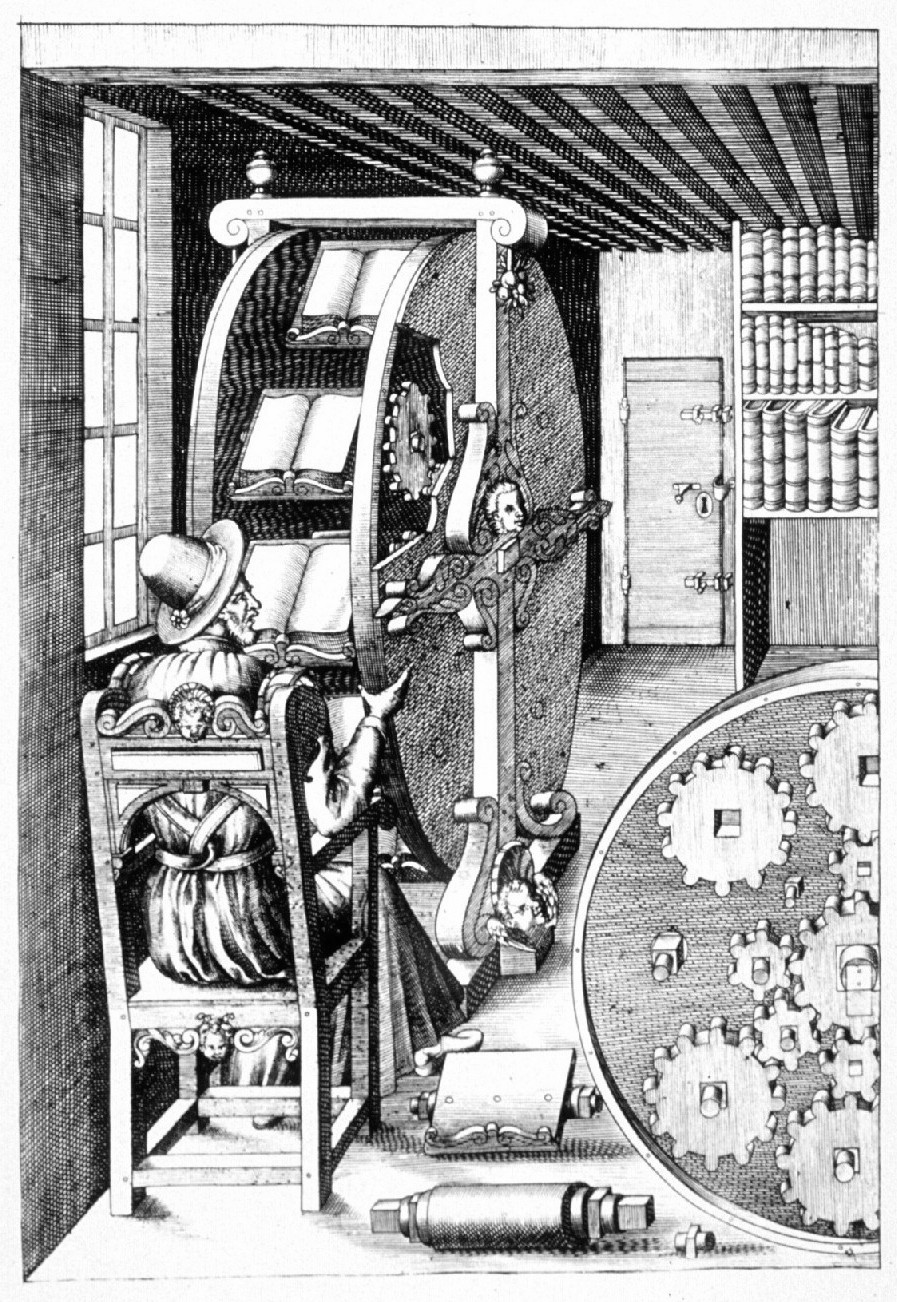
\includegraphics[width=.9\linewidth]{bookwheel.jpg}
\end{center}
\end{column}

\begin{column}{0.45\columnwidth}
\begin{itemize}
\item Structure and Interpretation of Computer Programs.
\item By Harold Abelson, Gerald J. Sussman and Julie Sussman.
\item 883 pages.
\item 353 problems.
\item No official solution.
\item Difficulty unknown.
\item Still cannot be solved portably.
\end{itemize}
\end{column}
\end{columns}
\end{frame}

\begin{frame}[label={sec:orge2b2c03}]{Who is this report for?}
\begin{itemize}
\item Teachers.
\item Teaching Assistants.
\item Self-learners.
\item Students.
\item Time-management enthusiasts.
\item Curriculum designers.
\end{itemize}
\end{frame}

\begin{frame}[label={sec:org0c3cdf8}]{Who I am. (Bias adjustment.)}
\begin{itemize}
\item Professional MATLAB developer.
\item PhD in Computer Science Theory.
\item MSc in Machine Learning.
\item BSc in Mathematics and Physics.
\item Studied C, C++, Python.
\end{itemize}
\end{frame}

\begin{frame}[label={sec:orgb99d260}]{What is perfect coursework solution artefact?}
\begin{itemize}
\item Plain text.
\item Version controlled.
\item Useful years later.
\item Useful on any machine.
\item Used as a portfolio.
\item Searchable.
\item Verifiable.
\end{itemize}
\end{frame}

\begin{frame}[label={sec:org0f56e4e}]{Which tools I used in the end.}
\end{frame}

\section{The Execution Process.}
\label{sec:org4c70654}

\begin{frame}[label={sec:orgc928092}]{Solving problems with babel.}
\end{frame}

\begin{frame}[label={sec:org0d9d16b}]{Graphical example.}
\end{frame}

\begin{frame}[label={sec:orga2442cb}]{Compiling the report.}
\end{frame}

\begin{frame}[label={sec:orgc52e8a9}]{Measuring time.}
\end{frame}

\begin{frame}[label={sec:orgb4dba3f}]{Motivational tricks.}
\end{frame}

\section{The Data and the Analysis.}
\label{sec:orgd0c028c}

\begin{frame}[label={sec:org48e5454}]{Statistics from outside org.}
\end{frame}

\begin{frame}[label={sec:org709e407}]{Data analysis with Emacs Lisp.}
\end{frame}

\begin{frame}[label={sec:org63ef066}]{Data demonstration.}
\end{frame}

\begin{frame}[label={sec:org3d840c8}]{Statistics graphs.}
\end{frame}

\section{Results and Conclusion.}
\label{sec:orgc508110}

\begin{frame}[label={sec:org2eebd5c}]{Hard problems to discuss.}
\end{frame}

\begin{frame}[label={sec:org82ed5f9}]{By-products of the work.}
\end{frame}

\begin{frame}[label={sec:org70bd427}]{Applications and Further Work.}
\end{frame}

\begin{frame}[label={sec:org52d2399}]{Review.}
\end{frame}

\begin{frame}[label={sec:orgb0b4a1c}]{Personal 1 minute.}
\end{frame}

\begin{frame}[label={sec:org37c6f5c}]{Credits.}
Contacts, gitlab, Patreon.
\end{frame}
\end{document}